\documentclass{article}
\usepackage{tikz}
\usetikzlibrary{patterns}

\begin{document}
	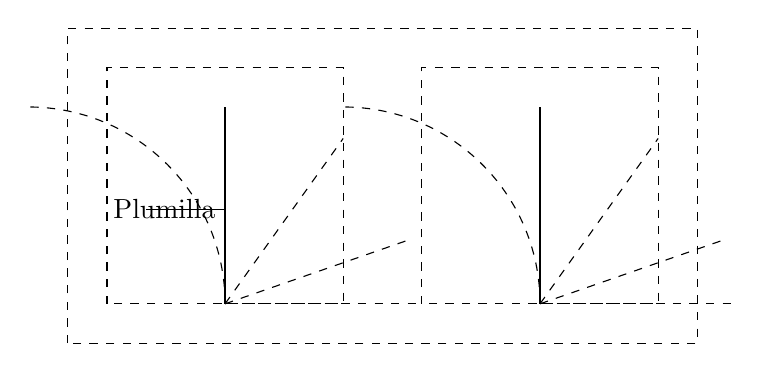
\begin{tikzpicture}
		
		% Rectángulo punteado que enmarca todo el diagrama (parabrisas completo)
		\draw[dashed] (0,0) rectangle (8,4);
		
		% Rectángulos punteados que enmarcan cada plumilla con su área de movimiento
		\draw[dashed] (0.5,0.5) rectangle (3.5,3.5);
		\draw[dashed] (4.5,0.5) rectangle (7.5,3.5);
		
		% Primera plumilla (izquierda)
		\begin{scope}[shift={(2,0.5)}]
			% Línea sólida vertical (plumilla en posición inicial)
			\draw[thick] (0,0) -- (0,2.5);
			
			% Trayectorias de movimiento (líneas punteadas)
			\draw[dashed] (0,0) -- (1.5,2.1);  % Trayectoria en ángulo 1
			\draw[dashed] (0,0) -- (2.3,0.8);  % Trayectoria en ángulo 2
			\draw[dashed] (0,0) -- (2.5,0);    % Trayectoria en ángulo 3
			
			% Arco punteado que muestra el rango de movimiento
			\draw[dashed] (0,0) arc (0:90:2.5);
			
			% Etiqueta "Plumilla" con línea que la señala
			\draw (0,1.2) node[left] {Plumilla} -- (-1,1.2);
		\end{scope}
		
		% Segunda plumilla (derecha)
		\begin{scope}[shift={(6,0.5)}]
			% Línea sólida vertical (plumilla en posición inicial)
			\draw[thick] (0,0) -- (0,2.5);
			
			% Trayectorias de movimiento (líneas punteadas)
			\draw[dashed] (0,0) -- (1.5,2.1);  % Trayectoria en ángulo 1
			\draw[dashed] (0,0) -- (2.3,0.8);  % Trayectoria en ángulo 2
			\draw[dashed] (0,0) -- (2.5,0);    % Trayectoria en ángulo 3
			
			% Arco punteado que muestra el rango de movimiento
			\draw[dashed] (0,0) arc (0:90:2.5);
		\end{scope}
		
	\end{tikzpicture}
\end{document}